\section{Principios de diseño}
Los principios de diseño (SOLID), la ley de Demeter, separación de incumbencias están siempre presentes en cada decisión que tomemos sobre la arquitectura.

Los criterios generales son:
\begin{itemize}
\item Economía
\item Visibilidad
\item 'Espaciamiento'
\item Simetría
\item Emergencias
\end{itemize}


\subsection*{Economía}
\begin{itemize}
\item Tiene que ver con el listado de métodos que componen una misma interfaz.
\item Busca evitar complejidades innecesarias, flexibilidad innecesaria, y enfocarnos en la usabilidad mas que en la reusabilidad.
\item La interfaz tiene que estar limpia y económica. Tener la mínima cantidad de métodos necesarios que sean útiles.
\end{itemize}


\subsection*{Visibilidad}

\begin{itemize}
\item La especificación en términos de interfaces y herencia o implementación suele ser obscura, poco visible y difícil de entender y navegar.
\item Es preferible la composición y delegación que la herencia.
\end{itemize}


\begin{figure}[!htb]
    \centering
    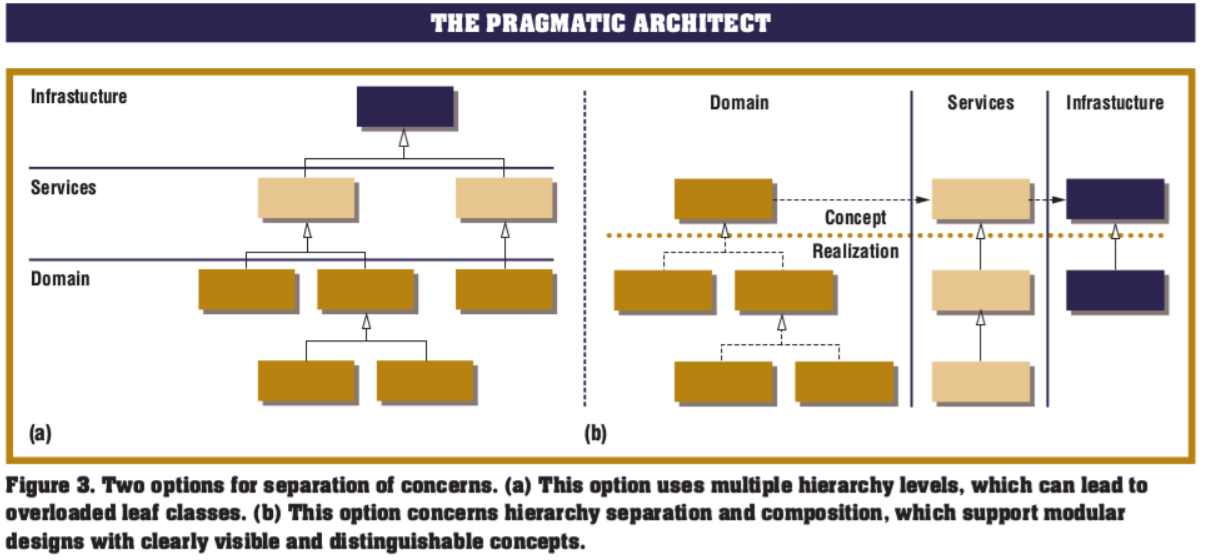
\includegraphics[width=0.8\textwidth]{img/VisibilidadPatrones.PNG}
\end{figure}

\subsection*{'Espaciamiento'}
\begin{itemize}
\item Tiene que ver con el desacoplamiento.
\item Contribuye a la visibilidad y el reuso.
\item Busca definir cuales son los roles de cada componente del diseño, lo cual nos ayuda a separarlos. Si nos cuesta definirlos es que esta en demasiadas cosas.
\item Distancia entre responsabilidades funcionales claramente distintas y autónomas conduce a componentes.
\item  Espaciado entre las perspectivas de uso de un componente conduce a interfaces con rol específico.
\item La separación entre grupos de componentes conduce a capas y subsistemas.
\item El espacio entre el contrato y la realización conduce a interfaces explícitas e implementaciones separadas.
\end{itemize}



\subsection*{Simetría}

\begin{itemize}
\item Facilita la comprensión, comunicación, extensión y mantenimiento.
\end{itemize}

\begin{figure}[!htb]
    \centering
    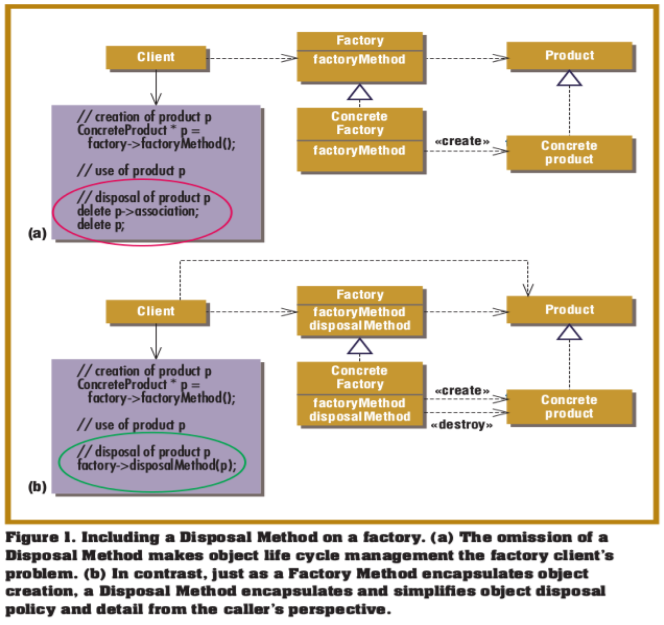
\includegraphics[width=0.8\textwidth]{img/simetriaPatrones.PNG}
    \caption{Diagrama de arriba se instancian instancias a través de un Factory que no destruye los objetos. Esto es asimétrico, solo crea no destruye.}
\end{figure}



\subsection*{Emergencias}
\begin{itemize}
\item Tiene que ver con algo que emerge por su forma, por su repetición en contexto similar.
\item Facilita la organización y escalabilidad.
\item Emergente es el comportamiento de auto-organización y junto con el control son a menudo la clave para la escalabilidad, eficiencia y economía en las arquitecturas
\end{itemize}


\section{Patrones}

\begin{itemize}
\item Situaciones que se empiezan a repetir y se puede solucionar de la misma forma.
\item Los definimos por un contexto en la cual se plantea un problema, el problema (\textit{que según Bushman puede estar compuesto por fuerzas que se contraponen y los patrones buscan balancear}), y por la solución (relación/interacción entre varias clases)
\item Nadie inventa patrones, estos se descubren.
\item Esta implícito en el nombre del patrón todo lo que constituye.
\item Son buena documentación de diseño.
\end{itemize}

\textit{Más adelante se sigue con patrones de diseño.}

\textit{Parte de donde surge la idea (arquitectura - de los edificios): A Pattern Language - Christopher Alexander }


\section{Patrones de arquitectura}
Para saber cuando usar cada uno, necesitamos saber el contexto y el problema que se presenta. Orientados a organizar la plataforma en la cual se va a construir el sistema.

\subsection*{Layer}

\begin{itemize}
\item Idea: Tenemos un sistema que tiene un volumen grande, en el cual aparecen conceptos de distinto nivel de abstracción.
\item Hay diferentes capas con distintos niveles de abstracción. \textit{Ej. Teléfonos presentado en clase, comunicación, tarifas de las llamadas, las impresoras, administración del locutorio} Cuando tenemos esto conviene el uso de este patrón.
\item Cada capa (layer) utiliza un servicio de la capa superior. Permite reutilizar partes.
\item Las ventajas son reuso, cambiabilidad, desarrollo simultaneo, ya que las capas se pueden manejar por separado.
\item La desventaja es un diseño mas elaborado
\item El patrón no ofrece una respuesta a cuantas capas tengo que tener, esto depende de los requerimientos. \textit{Ej. Modelo OSI de redes}
\end{itemize}

\begin{figure}[!htb]
    \centering
    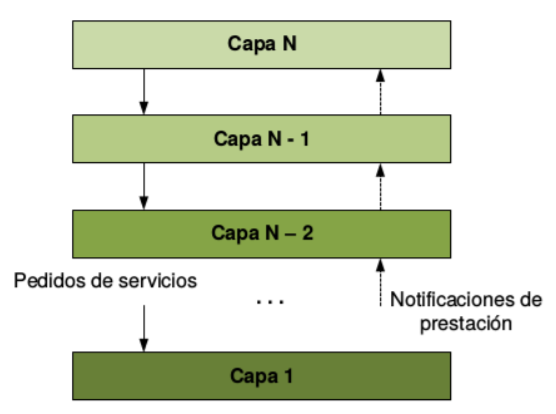
\includegraphics[width=0.8\textwidth]{img/LayerPatron.PNG}
\end{figure}

\subsection*{EA}
\begin{itemize}
\item Enterprise Architecture
\item Es un Mega patrón, compuesto por muchos patrones. (se va a ver mejor mas adelante)
\item Es conveniente usarlo cuando hay un sistema cliente-servidor (remoto). También cuando hay usuarios concurrentes, múltiples interfaces de usuario, reglas de negocio y datos persistentes.
\item Se usa desacoplando los diferentes 'tiers' para lograr separar incumbencias.
\item Las ventajas son el reuso y la cambiabilidad,
\item La desventaja es un mayor trabajo.
\end{itemize}


\begin{figure}[!htb]
    \centering
    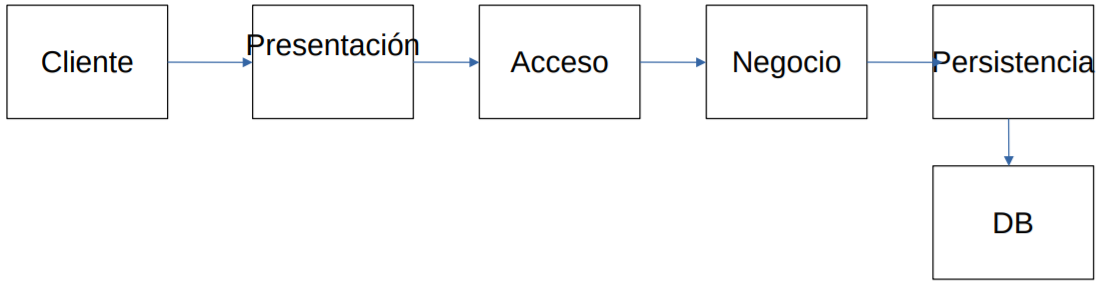
\includegraphics[width=0.8\textwidth]{img/EAPatron.PNG}
    \caption{Ejemplo}
\end{figure}


\subsection*{Microkernel}
El patrón arquitectónico de Microkernel se aplica a un sistema de software que debe ser capaz de adaptarse a los cambios en los requisitos del sistema. Separa un núcleo funcional mínimo de la funcionalidad extendida y de las piezas específicas del cliente. El microkernel también sirve como enchufe para conectar estas extensiones y coordinar su colaboración
\begin{itemize}
\item Conviene utilizarlo en sistemas de larga vida que deben evolucionar ante cambios de distinto tipo con diferente frecuencia.
\item Con un sistema monolítico se complica.
\item Asigna componentes esenciales al microkernel y distribuye las componentes entre los servers.
\item Esta compuesto por External Servers, el Microkernel, y el Internal Server
\item Las ventajas son que soporta cambios con menor impacto.
\item La desventaja es un diseño mas elaborado
\end{itemize}

\begin{figure}[!htb]
    \centering
    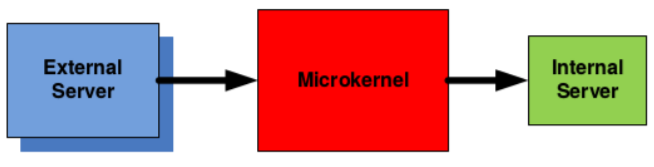
\includegraphics[width=0.8\textwidth]{img/MicrokernelPatron.PNG}
\end{figure}


\subsection*{Pipe Filter}

\begin{itemize}
\item Conviene usarlo cuando debemos procesar un stream de datos, y este procesamiento se puede descomponer en N procesamientos atómicos.
\item Permite sistemas mas reutilizables, es reuso.
\item Para usarlo, distribuir los procesamientos en filtros, definir el formato de datos en los pipes y definir la implementación.
\item La ventaja es el reuso y el rápido prototipado.
\item La desventaja es que no se puede usar en sistemas críticos ya que no podemos controlar el estado global. (en caso de que falle un filtro)
\end{itemize}

\begin{figure}[!htb]
    \centering
    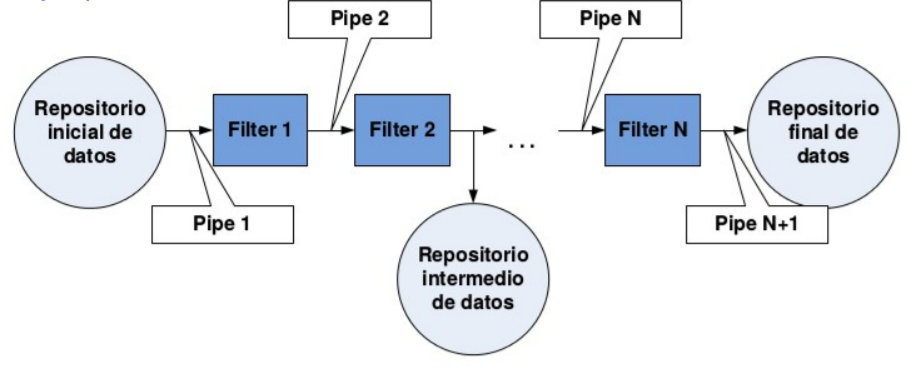
\includegraphics[width=0.8\textwidth]{img/PipeFilterPatron.PNG}
\end{figure}


\subsection*{MVC}

\begin{itemize}
\item Modelo-Vista-Controlador
\item Es conveniente usarlo cuando es necesario contar con interfaces de usuario múltiples y diferentes para los mismos datos, flexibles y cambiables.
\item El usuario solo interactúa con el modelo a través de los controladores.
\item El modelo esta desacoplado, se vuelve transportable.
\item Los ve en las vistas.
\item Viene de la mano con el patrón Observer, se encarga de propagar los cambios en el modelo.
\item La ventaja es la reusabilidad y facilidad de cambios y extensión
\item Las desventajas son que se tiene un mayor diseño y que hay que tener cuidado con las bibliotecas que ya implementan algo.
\end{itemize}

\begin{figure}[!htb]
    \centering
    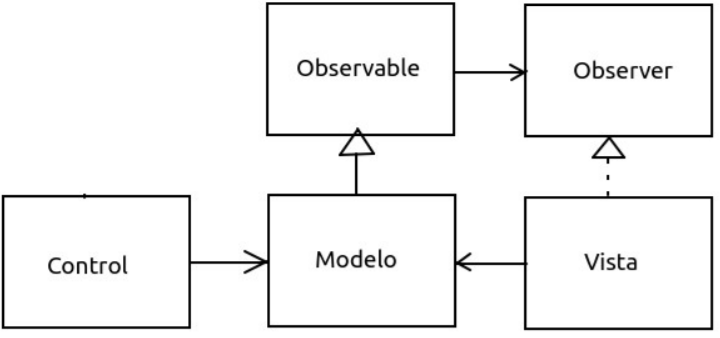
\includegraphics[width=0.7\textwidth]{img/MVCPatron.PNG}
\end{figure}

\subsection*{Broker}
El Broker es un patrón de arquitectura que se utiliza para estructurar sistemas de software distribuidos con componentes desacoplados que interactúan por invocaciones de servicios remotos. Esto quiere decir que, si un componente necesita un servicio de otro que está en otra ubicación que no conoce, el broker se encarga de proporcionar la conexión. Si los componentes manejaran la comunicación por sí mismos, el sistema se enfrentaría a diversas dependencias y limitaciones.
\begin{itemize}
\item Es necesario usarlo cuando se tiene que contar con procesamiento distribuido a partir de objetos distribuidos. También cuando es necesario abstraerse de la tecnología que implementa la comunicación entre procesos.
\item Conviene siempre que se pueda no distribuir los objetos.
\item Las ventajas son la cambiabilidad, la portabilidad, y el reuso.
\item Las desventajas son la baja eficiencia, dificultad de desarrollo y que no tolera fallas.
\item Esta compuesto por el Broker, dos proxies (Stub y Skeletor) que se ocupan de la serializacion e ida y vuelta.
\end{itemize}

\begin{figure}[!htb]
    \centering
    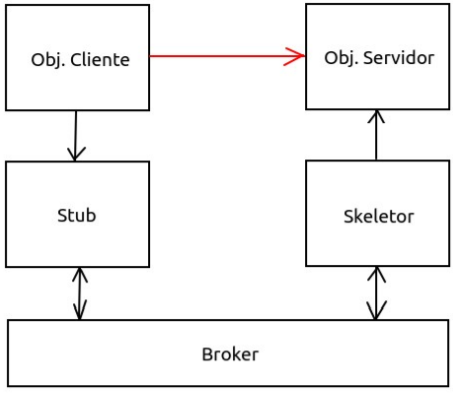
\includegraphics[width=0.5\textwidth]{img/BrokerPatron.PNG}
\end{figure}






